\documentclass{article}

%% Language and font encodings
\usepackage[english]{babel}
\usepackage[utf8x]{inputenc}
\usepackage[T1]{fontenc}
\usepackage{lmodern}
\usepackage{minted}
\usepackage{datatool}
\usepackage{nicefrac}


%% Sets page size and margins
\usepackage[letterpaper,top=1in,bottom=1in,left=1in,right=1in,marginparwidth=.5in]{geometry}

%% Useful packages
\usepackage{amsmath}
\usepackage{graphicx}
\usepackage[colorinlistoftodos]{todonotes}
\usepackage[colorlinks=true, allcolors=blue]{hyperref}

\graphicspath{{./images/}}

\title{World Happiness: Factors of Influence and Trajectory}
\author{Verro Ejiba, Meredith Miller, Youjin Zhang}

\begin{document}
\maketitle

\section{Introduction}
The 2017 World Happiness Report \cite{worldhappinessreport}, released on March 20, 2017, sought to globally measure happiness and understand the factors that might influence it, in order to aid policy makers in their decision-making process. The survey conducted by GWP (Gallup World Poll) collected data in 155 countries/territories and has been repeated yearly from 2005 through 2016. The happiness score, \texttt{life ladder} as recorded in the data, is the average response to survey answers asking respondents the Cantril Ladder question, i.e. “Please imagine a ladder, with steps numbered from 0 at the bottom to 10 at the top. The top of the ladder represents the best possible life for you and the bottom of the ladder represents the worst possible life for you. On which step of the ladder would you say you personally feel you stand at this time?” See Figure \ref{fig:long} for a visualization of world happiness, clustered by region.

The data set also contains 23 other variables on economic, social, and health aspects of each country. In this study, we sought to better understand the relationship between a country's happiness and the various predictor variables. Therefore, we explore two main models: 
\begin{enumerate}
	\item Classical linear regression: To model happiness against other economic, social, and health variables.
    \item Longitudinal mixed effects: To model happiness through time.
\end{enumerate}

\begin{figure}
\centering
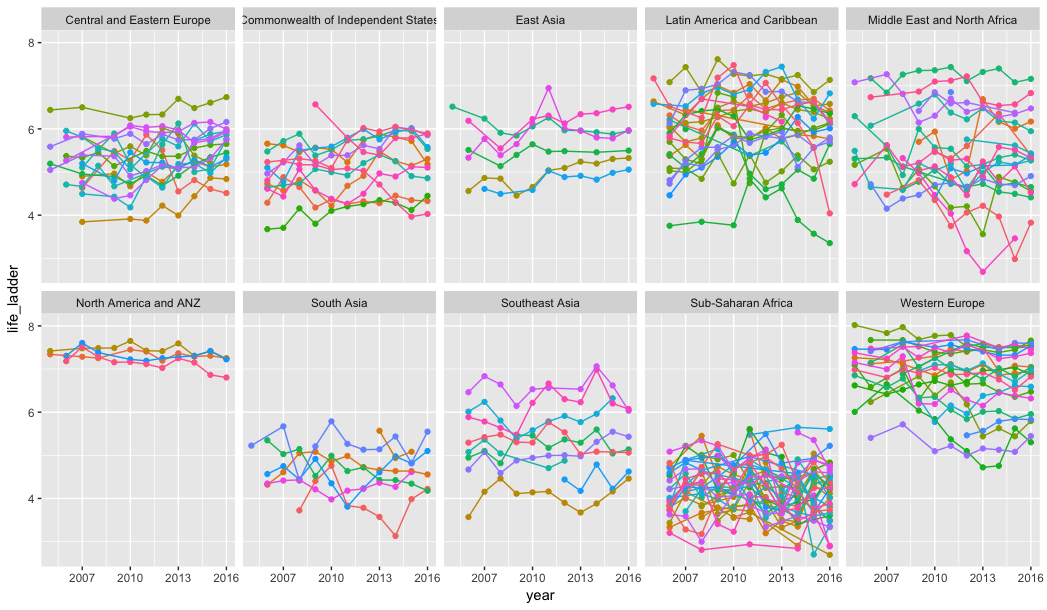
\includegraphics[scale=.45]{longitudinal.png}
\caption{\label{fig:long}Happiness score through the years, by World Region}
\end{figure}

The remainder of this analysis is organized as follows: Section \ref{sec:methods} discusses the methods used for both models; Section \ref{sec:results} describes the results from both analyses; and Section \ref{sec:discussion} discusses the overall results and next steps for analysis. Appendix \ref{sec:adx_derivations} includes full derivations and Appendix \ref{sec:adx_Rcode} contains all R code used in this study.

\section{Methods} \label{sec:methods}

\subsection{Classical Linear Regression Model}
We focused our analysis for this specific model in the year 2016, but a similar analysis can readily be done for other years. Also, out of the 23 explanatory variables, we limited our focus on the six most influential (as determined in the published report) and most consistently reported variables: log-GDP per capita, social support, healthy life expectancy, freedom of choice, generosity, and corruption perception.
Let $\boldsymbol{Y} = \left[Y_1, Y_2, ..., Y_n\right]^\mathsf{T}$ denote the response variable, \texttt{life ladder} as specified in the data and happiness score in the report, with $n$ being the number of countries sampled. Further, let $\boldsymbol{X} = \left[\mathbf{X}_{0},\mathbf{X}_{1}, \mathbf{X}_{2}, ..., \mathbf{X}_{6}\right]$ denote the design matrix including the six explanatory variables of interest and an intercept. Letting $\boldsymbol{\beta}$ be the vector of regression coefficients and $\sigma^2$ be the variance of model error, assumed to be uniform for simplicity. Thus the likelihood of the response variable, assuming normal distribution of model error, is:

\begin{equation} 
Y\sim MVN(\boldsymbol{X\beta}, \sigma^2\mathbf{I}_{(n,n)})
\end{equation}

We used a non-informative prior on $(\boldsymbol{\beta}, \sigma^2)$, which is appropriate for our regression model since we have many more data points, $n$ (i.e. 121 for 2016) than parameters, $k$ (i.e. 6). We then used a hierarchical model to determine the best-fit regression coefficients by alternately sampling from the full conditional of $\boldsymbol{\beta}$ and the marginal of $\sigma^2$. Finally, the prediction error, $e = Y - \tilde{Y}$, was computed using a hold-out set of the 2016 happiness data, by calculating the happiness predictions, $\tilde{Y}$, with the best-fit coefficients. \\

\subsection{Longitudinal Mixed Model}
Since the life ladder responses over the many years of the happiness survey constitute a prospective global study, we next conducted a longitudinal regression analysis, to predict each country's happiness trajectory. As seen in Figure \ref{fig:long}, the history of results vary widely by country, so we chose a mixed effects model with both random intercept and random slope(s). We limited this model to include only the time variable, $x$, with no other potential happiness predictors. We regressed happiness against time for the 10 happiest countries from the 2016 survey: Finland, Norway, Denmark, the Netherlands, Iceland, Switzerland, Sweden, Australia, Canada, and New Zealand.

We chose the years of 2008, 2012, 2013, 2014, 2015, and 2016 for our model, attempting to create near-complete cases. That is, the years of 2009 - 2011 had higher rates of missing data. We still retained four missing data points with the chosen years, where surveys were not conducted. This indicated that the values were missing completely at random, so we utilized simple imputation techniques, such as interpolation and nearest measured value \cite{gelman_hill_2016}. See Appendix \ref{sec:apx_long_data} for the final cleaned data set, with details of imputation.

Therefore, with each country indexed by $i$ and each year of observation indexed by $j$, we sought to model happiness, $y_{ij}$, according to Equation \ref{eqn:long_model} \cite{rolfe_2010}.
\begin{equation}
\begin{gathered} \label{eqn:long_model}
y_{ij}=\eta_{0i}+\eta_{1i}x_{ij}+\epsilon_{ij}, \quad \epsilon_{ij} \sim \mathcal{N} \left( 0, \nicefrac{1}{\tau_e^2} \right) \\\ 
\eta_{0i} = \beta_{0} + u_{0i}, \quad u_{0i} \sim \mathcal{N} \left( 0, \nicefrac{1}{\tau_{u0}^2} \right) \\
\eta_{1i} = \beta_{1} + u_{1i}, \quad u_{1i} \sim \mathcal{N} \left( 0, \nicefrac{1}{\tau_{u1}^2} \right) \\
\end{gathered}
\end{equation}

This leads to a multivariate normal likelihood for the response variable data as well as for the full set of country-specific random coefficients, $u_{0i}$ and $u_{1i}$. We used non-informative priors for the fixed regression coefficients, $\beta_0$ and $\beta_1$, and for the three precision parameters, $\tau_{e}^2$, $\tau_{u0}^2$, $\tau_{u1}^2$. Since this model results in a posterior from which we cannot readily sample, we chose a Gibbs Sampler with the full conditionals for the fixed and random regression coefficients and the three precision parameters of Equation \ref{eqn:long_model}. See Appendix \ref{sec:adx_long_deriv} for the detailed derivation of the posterior and full conditionals, and Appendix \ref{sec:adx_long_R} for the R code containing the Gibbs Sampler.

At every iteration of the sampler, we used the selected parameter values to predict the happiness score of each country for the survey to be taken in 2017. This allowed us to conduct posterior inference on questions of the predicted 2017 happiness by simply finding the frequency with which the the specified situation occurred. See Section \ref{sec:long_results} for specific question results. 

\section{Results} \label{sec:results}
\subsection{Classical Linear Regression Model}
See Table \ref{tab:summ} for a summary table of the parameter samples including the mean, median, and 95\% credible intervals. The density plots for each predictor variable can be seen in Figure \ref{fig:dist-basic} in Appendix \ref{sec:adx_extra}.

To test the assumption of normality of errors, we plotted the resulting density of errors following the regression, see Figure \ref{fig:pred}. Visual inspection of this density lends support to the assumption. Further assessments might include residual plots, normal Q-Q plots, and formal statistical tests. 

To determine the strength of the model fit, we computed the deviance information criterion (DIC), $R^2$, and the mean squared error (MSE), see Table \ref{tab:mod_ac}. The DIC is intended primarily as a reference point for comparison with potential future models, whereas the $R^2$ illustrates that much of the variance seen in happiness has been captured by the included predictors and indicates a strongly predictive model.

\begin{table}[h!]
\centering
\caption{\label{tab:summ} Summary of regression coefficients: mean, median, and credible intervals.}
\begin{tabular}{c c c c c c c c} \hline
Summary & Life ladder & logGDP & Social support & Healthy life & Free choice & Generosity & Corruption \\\hline
Mean & 5.384 & 0.378  & 2.509  & 0.027 & 1.680 & 0.989& -0.111\\
Median & 5.384 & 0.378 & 2.512 & 0.027 & 1.685 & 0.985 & -0.113\\
2.5\% & 5.285 & 0.195 &  1.255 & 0.002 & 0.735 & 0.225 & -0.780 \\
97.5\% & 5.487 & 0.564 & 3.744 & 0.052 & 2.598 & 1.741 & 0.547 \\\hline
\end{tabular} 
\end{table}

\begin{table} [h!]
\centering
\caption{\label{tab:mod_ac} Model checking and accuracy test: DIC, $R^{2}$, MSE.}
\begin{tabular}{c c c c} \hline
Test & DIC & $R^{2}$ & MSE \\\hline
Values & 225.343 & 0.867 & 0.245 \\
\end{tabular}
\end{table} 

\subsection{Longitudinal Mixed Model} \label{sec:long_results}
We ran the Gibbs Sampler for 20,000 iterations, checked convergence with running mean plots, and discarded half the samples for burn-in. The resulting parameters can be found in Table \ref{tab:long_params} and the fitted lines in Figure \ref{fig:each_long}. Note the wide credible intervals for the intercept parameters. This largely comes from the variance of the $\boldsymbol{\beta}$ sample, likely inflated due to the scale of the \texttt{year} data. Simply setting 2008 as a baseline year, valued at 0, should reduce this effect.

\begin{samepage}
To investigate the 2017 happiness predictions, we used our posterior draws to estimate the following probabilities:
\begin{enumerate}
	\item Finland continues to be the happiest country of the selected 10: 5.80\%
        \item Finland drops to the least happiest country of the selected 10: 1.86\%
    \item New Zealand overtakes Canada in happiness: 22.05\%
    \item Denmark will be the happiest country of the selected 10: 37.82\% (the highest of any country)
\end{enumerate}
\end{samepage}

\begin{table}[h!]
\centering
\caption{\label{tab:long_params}Mean Parameters and 95\% Credible Intervals, by Country}
\begin{tabular} {l}
\hline
    \DTLloaddb{long_final}{./data/output_long_params.csv}
	\DTLdisplaydb{long_final}
  \\ \hline
\end{tabular}
\end{table}

\begin{figure}[h!]
\centering
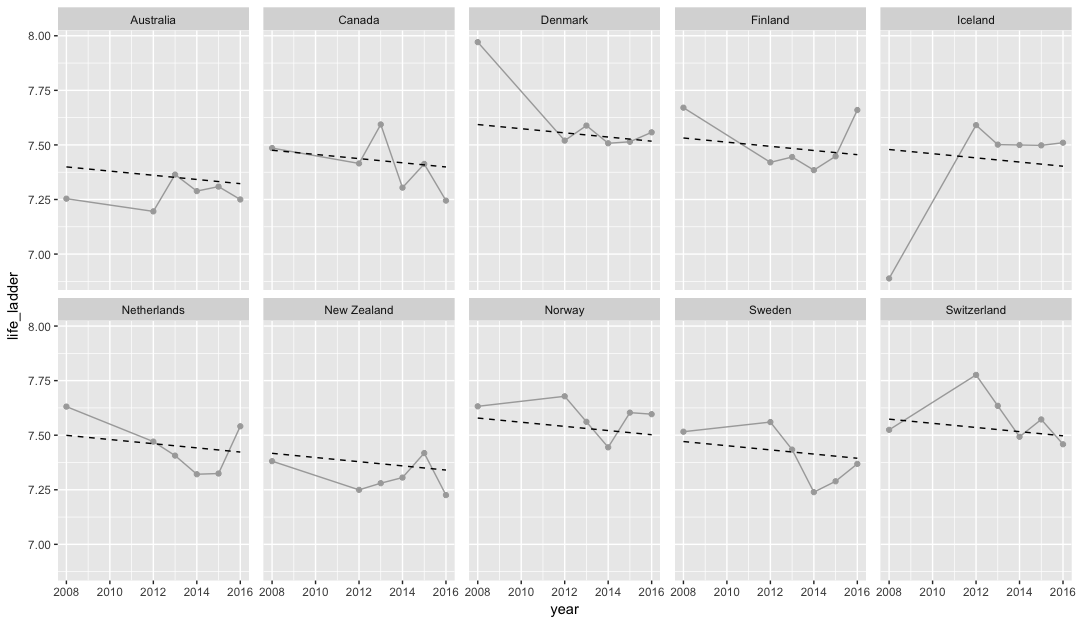
\includegraphics[scale=.45]{each_long_fit.png}
\caption{\label{fig:each_long}Longitudinal Regression Best-Fit Lines}
\end{figure}

\section{Discussion} \label{sec:discussion}
The linear regression model showed that the happiness score is positively affected by the GDP, healthy life expectancy, social support, freedom of choice, and lastly generosity and negatively affected by corruption. Therefore, global happiness seems to be influenced not only by economic status, but also largely by health and social life aspects. Next steps for this model might include using model selection priors, such as Laplacian (for LASSO) or normal (for ridge), utilizing results from previous years as prior information, and investigating ways to reduce the correlation of predictor variables (see Table \ref{tab:corr} in Appendix \ref{sec:adx_extra}).

The longitudinal mixed effects model illustrated that the top 10 happiest countries are tightly clustered, with seemingly stable happiness. For further analysis, this model could be extended to include more countries, more years (with further advanced methods of data imputation or by providing more model flexibility to handle missing data), time-invariant variables (such as world region), and more complex covariance structures among the the random effect coefficients.

\bibliographystyle{IEEEtran}
\bibliography{IEEEabrv,references}

\appendix

\section{Derivations} \label{sec:adx_derivations}

\subsection{Classical Linear Regression}
Assuming normality of the error term, $\epsilon$, we used a multivariate normal distribution to model the response variable, \texttt{life ladder}. Thus the likelihood of the response variable is, with $n$ observations:
\begin{equation*} 
\mathbf{Y}\sim MVN(\boldsymbol{X\beta}, \sigma^2\mathbf{I}_{(n,n)})
\end{equation*}
with the error term assumed to be normal, $\epsilon \sim MVN(0, \sigma^2\mathbf{I_{(n,n)}})$.

Using a non-informative prior on $\beta$ and $\sigma^2$, we have that:
\begin{equation*}
p(\boldsymbol{\beta}, \sigma^2) \propto \left(\sigma^2\right)^{-1}
\end{equation*}

The marginal posterior on $\sigma^2$ is defined as:
\begin{equation*}
\sigma^2 \mid \mathbf{Y} \sim Inv-\chi^2(n-k, s^2)
\end{equation*}
where $s^2 = \frac{1}{n-k}(\mathbf{Y} - \mathbf{X}\hat{\boldsymbol{\beta}})^{\mathsf{T}}(\mathbf{Y} - \mathbf{X}\hat{\boldsymbol{\beta}})$ and $\hat{\boldsymbol{\beta}} = (\mathbf{X}^{\mathsf{T}}\mathbf{X})^{-1}(\mathbf{X}^{\mathsf{T}}\mathbf{Y})$

Then the full conditional on $\boldsymbol{\beta}$ is:
\begin{equation*}
\boldsymbol{\beta} \mid \sigma^2, \mathbf{Y} \sim MVN(\hat{\boldsymbol{\beta}}, \mathbf{V}_{\beta}\sigma^2)
\end{equation*}
with $\mathbf{V}_{\beta} = (\mathbf{X}^{\mathsf{T}}\mathbf{X})^{-1}$

Thus, the posterior is defined as the product of the full conditional of $\boldsymbol{\beta}$ and the marginal of $\sigma^2$:
\begin{equation*}
p(\boldsymbol{\beta}, \sigma^2 \mid \mathbf{Y}) \propto p(\boldsymbol{\beta} \mid \sigma^2, \mathbf{Y}) p(\sigma^2 \mid \mathbf{Y})
\end{equation*}

\subsection{Longitudinal Mixed Effects Model} \label{sec:adx_long_deriv}
To model the individual country happiness responses over the yearly changes, we used a mixed effects model with group and individual effects on the intercept and slope. For simplification, we used time as the only predictor variable, $x$, and assume that the between-subject variability are normally distributed and independent of each other, for simplicity. That is, if each country is indexed by $i$ and each year of observation is indexed by $j$, then the response variable, $y_{ij}$ is modeled as \cite{rolfe_2010}:

\begin{gather*} 
y_{ij}=\eta_{0i}+\eta_{1i}x_{ij}+\epsilon_{ij}, \quad \epsilon_{ij} \sim \mathcal{N} \left( 0, \frac{1}{\tau_e^2} \right) \\ 
\eta_{0i} = \beta_{0} + u_{0i}, \quad u_{0i} \sim \mathcal{N} \left( 0, \frac{1}{\tau_{u0}^2} \right) \\
\eta_{1i} = \beta_{1} + u_{1i}, \quad u_{1i} \sim \mathcal{N} \left( 0, \frac{1}{\tau_{u1}^2} \right) \\
\end{gather*}

Above, we denote the fixed effects through the $\beta$ parameters, the random effects through the $u$ parameters, and the model errors through the $\epsilon$ parameters. Representing this model in matrix notation, with $n$ being the total number of countries and $T$ being the total number of sampling years, we have that:
\begin{equation} \label{eqn:adx_longmodel}
\mathbf{Y}=\mathbf{X}\boldsymbol{\beta}+\mathbf{ZU}+\mathbf{E}
\end{equation}
Letting
\begin{gather*}
\mathbf{X_{i}}=
\begin{bmatrix}
    1 & x_{i1} \\ 
    1 & x_{i2} \\ 
  	\vdots & \vdots\\ 
    1 & x_{iT}
\end{bmatrix}, \quad
\mathbf{Y_i}=
\begin{bmatrix}
    y_{i1} \\ 
    y_{i2} \\ 
  	\vdots \\ 
    y_{iT}
\end{bmatrix}, \quad
\mathbf{U_i}=
\begin{bmatrix}
    u_{0i} \\ 
    u_{1i}
\end{bmatrix}, \quad
\mathbf{E_i}=
\begin{bmatrix}
    e_{i1} \\ 
    e_{i2} \\ 
  	\vdots \\ 
    e_{iT}
\end{bmatrix}
\end{gather*}

we define
\begin{gather*}
\mathbf{Y} = 
\begin{bmatrix}
    \mathbf{Y_1} \\ \mathbf{Y_2} \\ \vdots \\ \mathbf{Y_n}
\end{bmatrix},
\quad
\mathbf{X}=
\begin{bmatrix}
    \mathbf{X_{1}} \\ \mathbf{X_{2}} \\ \vdots \\ \mathbf{X_{n}}
\end{bmatrix},
\quad
\boldsymbol{\beta} = 
\begin{bmatrix}
    \beta_{0} \\ \beta_{1} 
\end{bmatrix}, \\
\mathbf{Z} = 
\begin{bmatrix}
    \mathbf{X_{1}} & 0 & \hdots & 0 \\
    0 & \mathbf{X_{2}} & \hdots & 0 \\
  	\vdots & \vdots & \ddots & \vdots \\ 
    0 & 0 & \hdots & \mathbf{X_{n}}
\end{bmatrix},
\quad
\mathbf{U} = 
\begin{bmatrix}
    \mathbf{U_1} \\ \mathbf{U_2} \\ \vdots \\ \mathbf{U_n}
\end{bmatrix},
\quad
\mathbf{E} = 
\begin{bmatrix}
    \mathbf{E_1} \\ \mathbf{E_2} \\ \vdots \\ \mathbf{E_n}
\end{bmatrix}
\end{gather*}

With this set-up, we see that all the terms on the right-hand side of Equation \ref{eqn:adx_longmodel} resolve to vectors of length $nT$, the total number of observations:
\begin{itemize}
	\item $\mathbf{X}$ is $(nT,2)$
    \item $\boldsymbol{\beta}$ is $(2,1)$
    \item $\mathbf{Z}$ is $(nT,2n)$
    \item $\mathbf{U}$ is $(2n,1)$
    \item $\mathbf{E}$ is $(nT,1)$
\end{itemize}

We now assume that $\mathbf{Y} \sim MVN \left( \mathbf{X}\boldsymbol{\beta}+\mathbf{ZU}, \left( \tau_e^2 \right)^{-1} \mathbf{I}_{(nT,nT)} \right)$. We further choose to use the following priors:

\begin{itemize}
	\item $\pi \left( \boldsymbol{\beta}, \tau_e^2 \right) \propto \left( \tau_e^2 \right) ^{-1}$
    \item $\mathbf{U} \sim MVN \left( \mathbf{0}, \boldsymbol{\Sigma} \right)$, where the $(2n,2n)$ covariance matrix is
$$\boldsymbol{\Sigma} = \begin{bmatrix}
    \boldsymbol{\tau} & 0 & \hdots & 0 \\
    0 & \boldsymbol{\tau}  & \hdots & 0 \\
  	\vdots & \vdots & \ddots & \vdots \\ 
    0 & 0 & \hdots & \boldsymbol{\tau} 
\end{bmatrix},
\quad
\boldsymbol{\tau} = 
\begin{bmatrix}
    \frac{1}{\tau_{u0}^2} & 0 \\ 
    0 &  \frac{1}{\tau_{u1}^2}
\end{bmatrix}
$$
    \item $\pi \left( \tau_{u0}^2 \right) \propto \left( \tau_{u0}^2 \right) ^{-1}$
    \item $\pi \left( \tau_{u1}^2 \right) \propto \left( \tau_{u1}^2 \right) ^{-1}$
\end{itemize}

Therefore, the full posterior is

\begin{align*}
p \left( \boldsymbol{\beta}, \tau_e^2, \mathbf{U}, \tau_{u0}^2, \tau_{u1}^2 \mid \mathbf{Y} \right) & \propto \left( \tau_e^2 \right)^{\frac{nT}{2}} \exp \left[ -\frac{\tau_e^2}{2} \left( \mathbf{Y} - \left( \mathbf{X}\boldsymbol{\beta}+\mathbf{ZU} \right) \right)^{\mathsf{T}} \left( \mathbf{Y}- \left( \mathbf{X}\boldsymbol{\beta}+\mathbf{ZU} \right) \right) \right] \\
&\qquad \left( \tau_{u0}^2 \right)^{\frac{n}{2}} \left( \tau_{u1}^2 \right)^{\frac{n}{2}} \exp \left[-\frac{1}{2} \left( \mathbf{U} \right)^{\mathsf{T}}\boldsymbol{\Sigma}^{-1}\left(\mathbf{U} \right) \right] \left( \tau_{e}^2 \right)^{-1} \left( \tau_{u0}^2 \right)^{-1} \left( \tau_{u1}^2 \right)^{-1} \\
&= \left( \tau_e^2 \right)^{\frac{nT}{2}-1} \left( \tau_{u0}^2 \right)^{\frac{n}{2}-1} \left( \tau_{u1}^2 \right)^{\frac{n}{2}-1} \\
&\qquad \exp \left[ -\frac{\tau_e^2}{2} \left( \mathbf{Y} - \left( \mathbf{X}\boldsymbol{\beta}+\mathbf{ZU} \right) \right)^{\mathsf{T}} \left( \mathbf{Y}- \left( \mathbf{X}\boldsymbol{\beta}+\mathbf{ZU} \right) \right) \right]   \exp \left[-\frac{1}{2} \left( \mathbf{U} \right)^{\mathsf{T}}\boldsymbol{\Sigma}^{-1}\left(\mathbf{U} \right) \right]
\end{align*}

We now seek the full conditionals, to facilitate a Gibbs Sampler to generate samples from the posterior. By fixing all parameters but $\tau_{u0}^2$ in the posterior, we find:

\begin{align*}
	p \left( \tau_{u0}^2 \mid \boldsymbol{\beta}, \tau_e^2, \mathbf{U}, \tau_{u1}^2, \mathbf{Y} \right) &\propto \left( \tau_{u0}^2 \right)^{\frac{n}{2}-1}  \exp \left[-\frac{1}{2} \left( \mathbf{U} \right)^{ \mathsf{T}}\boldsymbol{\Sigma}^{-1} \left( \mathbf{U} \right) \right] \\
    &= \left( \tau_{u0}^2 \right)^{\frac{n}{2}-1}  \exp \left[-\frac{1}{2}  \tau_{u0}^2 \sum_{i=1}^{n} u_{0i}^2 \right]
\end{align*}

$$\tau_{u0}^2 \mid \mathbf{U}, \boldsymbol{\beta}, \tau_e^2, \tau_{u1}^2, \mathbf{Y} \sim \mathrm{Gamma} \left( \frac{n}{2}, \frac{1}{2} \sum_{i=1}^{n} u_{0i}^2 \right)$$

Similarly,

$$\tau_{u1}^2 \mid \mathbf{U}, \boldsymbol{\beta}, \tau_e^2, \tau_{u0}^2, \mathbf{Y} \sim \mathrm{Gamma} \left( \frac{n}{2}, \frac{1}{2} \sum_{i=1}^{n} u_{1i}^2 \right)$$

For the full conditional of $\boldsymbol{\beta}$:

\begin{align*}
p \left( \boldsymbol{\beta} \mid \tau_e^2, \mathbf{U}, \tau_{u0}^2, \tau_{u1}^2, \mathbf{Y} \right) &\propto \exp \left[ -\frac{\tau_e^2}{2} \left( \mathbf{Y} - \left( \mathbf{X}\boldsymbol{\beta}+\mathbf{ZU} \right) \right)^{\mathsf{T}} \left( \mathbf{Y}- \left( \mathbf{X}\boldsymbol{\beta}+\mathbf{ZU} \right) \right) \right] \\
&= \exp \left[ -\frac{\tau_e^2}{2} \left( \left( \mathbf{Y} - \mathbf{ZU} \right) - \mathbf{X}\boldsymbol{\beta} \right)^{\mathsf{T}} \left( \left( \mathbf{Y} - \mathbf{ZU} \right) - \mathbf{X}\boldsymbol{\beta} \right) \right]
\end{align*}

Noting the similarities with the standard regression conditional, i.e. the traditional response variable vector is now replaced with $\left( \mathbf{Y} - \mathbf{ZU} \right)$, we can let
$$\hat{\boldsymbol{\beta}} = \left(\mathbf{X}^{\mathsf{T}}\mathbf{X}\right)^{-1}\mathbf{X}^{\mathsf{T}}\left( \mathbf{Y} - \mathbf{ZU} \right)$$

so that

$$\boldsymbol{\beta} \mid \tau_e^2, \mathbf{U}, \tau_{u0}^2, \tau_{u1}^2, \mathbf{Y} \sim MVN \left[ \hat{\boldsymbol{\beta}}, \frac{1}{\tau_e^2} \left( \mathbf{X}^\mathsf{T} \mathbf{X} \right)^{-1} \right]$$

Using the same substitution, we know that

$$\tau_e^2 \mid \mathbf{U}, \boldsymbol{\beta}, \tau_{u0}^2, \tau_{u1}^2, \mathbf{Y} \sim \mathrm{Gamma} \left[ \frac{nT}{2}, \frac{1}{2} \left( \mathbf{Y}-\mathbf{X}\boldsymbol{\beta} - \mathbf{ZU} \right)^\mathsf{T} \left( \mathbf{Y}-\mathbf{X}\boldsymbol{\beta} - \mathbf{ZU} \right) \right]$$

To find the full conditional on $\mathbf{U}$, we must expand and combine the two exponential terms of the posterior.

\begin{align*}
p \left( \mathbf{U} \mid \boldsymbol{\beta}, \tau_e^2, \tau_{u0}^2, \tau_{u1}^2, \mathbf{Y} \right) &\propto \exp \left[ -\frac{\tau_e^2}{2} \left( \left( \mathbf{Y} - \mathbf{ZU} \right) - \mathbf{X}\boldsymbol{\beta} \right)^{\mathsf{T}} \left( \left( \mathbf{Y} - \mathbf{ZU} \right) - \mathbf{X}\boldsymbol{\beta} \right) \right] \exp \left[-\frac{1}{2} \left( \mathbf{U} \right)^{\mathsf{T}}\boldsymbol{\Sigma}^{-1}\left(\mathbf{U} \right) \right] \\
\begin{split}
&= \exp \left[ -\frac{1}{2} \left\lbrace \tau_e^2 \left( \mathbf{Y} - \mathbf{X}\boldsymbol{\beta} \right)^{\mathsf{T}} \left( \mathbf{Y} - \mathbf{X}\boldsymbol{\beta} \right) - \tau_e^2 \left( \mathbf{Y} - \mathbf{X}\boldsymbol{\beta} \right)^{\mathsf{T}} \left( \mathbf{ZU} \right) \right. \right. \\ & \qquad \qquad \qquad \left. \left. - \tau_e^2 \left( \mathbf{ZU} \right)^{\mathsf{T}} \left( \mathbf{Y} - \mathbf{X}\boldsymbol{\beta} \right) + \tau_e^2 \left( \mathbf{ZU} \right)^{\mathsf{T}} \left( \mathbf{ZU} \right) + \mathbf{U}^{\mathsf{T}}\boldsymbol{\Sigma}^{-1}\mathbf{U}  \right\rbrace \right]
\end{split} \\
&\propto \exp \left[ -\frac{1}{2} \left\lbrace - 2\tau_e^2 \left( \mathbf{Y} - \mathbf{X}\boldsymbol{\beta} \right)^{\mathsf{T}}\mathbf{ZU} + \mathbf{U}^{\mathsf{T}} \left( \tau_e^2 \mathbf{Z}^{\mathsf{T}}\mathbf{Z} + \boldsymbol{\Sigma}^{-1} \right) \mathbf{U}  \right\rbrace \right]
\end{align*}

Therefore, after completing the square, we find that the conditional is:

$$\mathbf{U} \mid \boldsymbol{\beta}, \tau_e^2, \tau_{u0}^2, \tau_{u1}^2, \mathbf{Y} \sim MVN \left[ \tau_e^2 \left( \tau_e^2 \mathbf{Z}^\mathsf{T} \mathbf{Z} + \boldsymbol{\Sigma}^{-1} \right)^{-1} \mathbf{Z}^\mathsf{T} \left( \mathbf{Y}-\mathbf{X}\boldsymbol{\beta} \right), \left( \tau_e^2 \mathbf{Z}^\mathsf{T} \mathbf{Z} + \boldsymbol{\Sigma}^{-1} \right)^{-1} \right]$$

\section{R code} \label{sec:adx_Rcode}

\subsection{Data Cleaning and Exploration}
\begin{minted}[mathescape,gobble=0,fontsize=\small]{R}
require(readr)
require(readxl)
require(dplyr)
require(ggplot2)

#GENERAL IMPORT AND CLEANING

# Load in main data source & rename columns
happiness <- read_excel("online-data-chapter-2-whr-2017.xlsx", 
                        sheet = "Data behind Table 2.1 WHR 2017")
happiness_names <- c("wp5_country","country","year","life_ladder",
                     "log_gdp_percapita","social_support","healthy_life_expectancy",
                     "freedom_of_choice","generosity","corruption_perception",
                     "positive affect","negative affect","govt_confidence",
                     "democratic_quality","delivery_quality","sd_lifeladder",
                     "sd_over_mean_lifeladder","gini_ind","gini_ind_avg",
                     "gine_house_income","trust_gallup","trust_81to84",
                     "trust89to93","trust94to98","trust99to04",
                     "trust05to09","trust10to14")
happiness <- as_data_frame(happiness)
colnames(happiness) <- happiness_names

# Load in data source with regional labels
regions <- read_delim("regions.csv", delim=",")
colnames(regions) <- c("region", "country")

# Join the main data set with the regional labels,
# Extract another data set with just 2016
hap_df <- left_join(happiness, regions, by='country')
hap2016 <- filter(hap_df, year=="2016")

# DATA EXPLORATION AND VISUALIZATION
# Plot longitudinal data
ggplot(data=hap_df, mapping=aes(x=year,y=life_ladder)) +
  geom_point(aes(color=wp5_country),show.legend=FALSE) +
  geom_line(aes(color=wp5_country),show.legend=FALSE) +
  facet_wrap(~ region, nrow=2)

# Plot pairs of predictors and response variables
pairs(hap2016[,c(4:7)])
pairs(hap2016[,c(4,8:10)])
pairs(hap2016[,c(4,11:13)])

# PREPARE DATA FOR LONGITUDINAL ANALYSIS
# First we reshape the data to ensure observations in
# the same years across countries

# This interpolates the life_ladder data from 2012, 2014
# for Norway and Switzerland to populate a value for 2013
i2013 <- happiestAll %>%
  filter(country %in% c("Norway","Switzerland")) %>%
  filter(year %in% c(2012,2014)) %>%
  group_by(country) %>%
  dplyr::summarize(life_ladder=mean(life_ladder)) %>%
  cbind(year=rep(2013,2)) %>%
  cbind(region=rep("Western Europe",2)) %>%
  dplyr::select(country,year,life_ladder,region)

# This interpolates the life_ladder data from 2013, 2015
# for Iceland to populate a value for 2014
i2014 <- happiestAll %>%
  filter(country == "Iceland") %>%
  filter(year %in% c(2013,2015)) %>%
  group_by(country) %>%
  dplyr::summarize(life_ladder = mean(life_ladder)) %>%
  cbind(year=2014) %>%
  cbind(region="Western Europe") %>%
  dplyr::select(country,year,life_ladder,region)
  
# This binds the observed data with the generated
# observations from above and with 
# taking the 2009 Switzerland value
# for 2008, to complete the data set
happiestAug <- happiestAll %>% 
  rbind(c(country="Switzerland",year=2008,
          happiestAll[happiestAll$country=="Switzerland" & happiestAll$year==2009,"life_ladder"],
          region="Western Europe")) %>%
  rbind(i2013) %>%
  rbind(i2014) %>%
  filter(year %in% c(2008,2012,2013,2014,2015,2016)) %>%
  arrange(country, year)

# Output the cleaned data set as wide format CSV
happiestAug_wide <- happiestAug %>% 
  spread(key=year,value=life_ladder) %>%
  arrange(desc(`2016`)) %>%
  dplyr::select(Country=country,Region=region,everything())
write_csv(format(happiestAug_wide, digits=3, nsmall=2),"happiest_clean.csv")
\end{minted}

\subsection{Classical Linear Regression}
\begin{minted}[mathescape,gobble=0,fontsize=\small]{R}
controller <- function(X,y,B) {
  set.seed(414)
  r <- regress(X, y, B)
  
  # Burn-in done by the regress function
  # Convergence
  rm <- apply(r$coeff,2,function(x) (cumsum(x)/(1:length(x)))-mean(x))
  
  # Summary
  s <- summary_coeff(r$coeff)
  
  # Capture densities
  all_d <- apply(r$coeff,2,density)
  
  return(list(regress=r, converge=rm, summary=s, densities=all_d))
}

norm <- function(x) {
  return(sum(x^2))
}

rinvchisq <- function(n,v,s2) {
  return(rinvgamma(n,v/2,v*s2/2))
}

# Extract data components, center each column
regress <- function(X,y,B) {
  require(mvtnorm)
  require(MCMCpack)
  
  # Determine parameters
  sizes <- dim(X)
  n <- sizes[1]
  k <- sizes[2]+1
  nk <- n-k
  
  # Initialize storage
  beta_mat <- matrix(NA, nrow = B, ncol = k)
  sigma2_vec <- rep(NA,B)
  
  # Prepare data structures
  X <- apply(X, 2, function(x) x - mean(x)) # Center data
  X <- cbind(intercept = rep(1,n),X) # Add intercept column
  colnames(beta_mat) <- colnames(X)
  
  XTy <- t(X)%*%y
  V_beta <- solve(t(X)%*%X)
  beta_hat <- V_beta%*%XTy
  s2 <- norm(y-X%*%beta_hat)/nk
  
  # Sample from Joint
  for (i in 1:B) {
    sigma2_vec[i] <- rinvchisq(1,nk,s2)
    beta_mat[i,] <- rmvnorm(1,beta_hat,V_beta*sigma2_vec[i])
  }
  return(list(dmat=X,coeff=beta_mat[((B/2)+1):B,],variance=sigma2_vec[((B/2)+1):B]))
}

summary_coeff <- function(coeff_mat) {
  m1 <- apply(coeff_mat,2,mean)
  m2 <- apply(coeff_mat,2,median)
  ci <- apply(coeff_mat,2,quantile,probs=c(0.025,0.975))
  s <- rbind(mean=m1, median=m2, ci)
  return(s)
}

plot_dist <- function(title,credInt,d) {
  plot(d,col='blue',xlab='Value',main=title)
  idStart <- max(which(d$x < credInt[1])) + 1
  idEnd <- min(which(d$x > credInt[2])) - 1
  gx <- d$x[idStart:idEnd]
  gy <- d$y[idStart:idEnd]
  px <- rep(0, length(gy))
  polygon(c(gx, rev(gx)), c(px, rev(gy)), border = FALSE,
          col = rgb(0, 0, 1, alpha = 0.5))
}

dic_norm <- function(y,results) {
  # Extract needed variables
  all_beta <- results$regress$coeff
  beta_mean <- results$summary[1,]
  dmat <- results$regress$dmat
  sig2 <- results$regress$variance
  y <- matrix(y,nrow=1)
  
  # Computer mean parameters
  I <- diag(length(y))
  mu_mean <- dmat%*%matrix(beta_mean,ncol=1)
  sigma_mean <- sqrt(mean(sig2))*I
  
  lik_mean <- dmvnorm(y,mean=mu_mean,sigma=sigma_mean,log=TRUE)
  
  # Initialize storage
  B <- length(sig2)
  ylik <- rep(NA,B)
  
  # Compute likelihood at each sample
  for (i in 1:B) {
    b <- matrix(all_beta[i,],ncol=1)
    s <- sig2[i]
    ylik[i] <- dmvnorm(y,mean=dmat%*%b,sigma=sqrt(s)*I,log=TRUE)
  }
  pdic <- 2*(lik_mean-(sum(ylik)/B))
  DIC <- -2*lik_mean+2*pdic
  return(DIC)
}

# MAIN REGRESSION CALLS
# Subset data
hap_2016_r <- hap2016[,c('life_ladder','log_gdp_percapita','social_support',
                         'healthy_life_expectancy','freedom_of_choice',
                         'generosity','corruption_perception')]
# Set initial parameters
B <- 20000

hap_2016_r <- hap_2016_r[complete.cases(hap_2016_r),]
cor(hap_2016_r)

y <- as.matrix(hap_2016_r[,1])
X <- hap_2016_r[,-1]

results <- controller(X,y,B)
results$summary

# Burn-in is done in the regress function output
# Plot convergence
par(mfrow=c(1,1))
matplot(results$converge,type='l',ylim=c(-0.1,0.1),
        ylab='Running Mean')

# Plot regression parameter distributions
par(mfrow=c(3,2))
lnames <- names(results$densities)
for (i in 2:7) {
  plot_dist(lnames[i],results$summary[3:4,i],results$densities[[i]])
}

# Compute DIC
dic <- dic_norm(y,results)
dic


## Cross Validation -- Holdout set for posterior prediction ##
library(pls)
# Randomly separate the data set into 2 groups
train <- sample(1:nrow(hap_2016_r),nrow(hap_2016_r)/2)
# Assign first half to training set and second half to holdout set
hap_test <- hap_2016_r[complete.cases(-train),]
olm_train <- hap_test[train,]
dim(olm_train)
olm_test <- hap_test[-train,]
dim(olm_test)
## Regression model for the holdout set 
test_res <- controller(olm_test[,-1], as.matrix(olm_test[,1]), B)
## Regression model for the training set 
ytrain <- as.matrix(olm_train[,1])
xtrain <- olm_train[,-1]
train_res <- controller(xtrain, ytrain, B)
train_res$summary
pred_res <- controller(train_res$regress$coeff[,-1], train_res$regress$coeff[,1], B)
ytild <- pred_res$regress$coeff[,1] #Prediction, Ytilda
y_test <- test_res$regress$coeff[,1]
#Prediction error
e <- y_test - ytild
# Calculate MSE
mean((y_test - ytild)^2)
#plot for residual
par(mfrow=c(1,2))
plot(density(e), main = "Density Plot of the Residual, error term")
plot(e, main = "Plot of the Error Parameter")
#Compute the R^2
mu <- test_res$regress$coeff[,-1]\%*\%matrix(test_res$summary[1,-1]) #mean matrix
ss_tot <- sum((y_test - mu)^2)
ss_reg <- sum((ytild - mu)^2) #Regression sum of squares
ss_res <- sum(e^2)
R2 <- 1-ss_res/ss_tot
R2

\end{minted}

\subsection{Longitudinal Mixed Effects Model} \label{sec:adx_long_R}
\begin{minted}[mathescape,gobble=0,fontsize=\small]{R}
# --------------------------------------------------------------------
# Longitudinal Mixed Model Work
# --------------------------------------------------------------------
# REQUIRES: cleaned data set: happiestAug
require(MCMCpack)
require(mvtnorm)
require(Matrix)

# Function to summarize based on column vectors
summary_coeff_row <- function(coeff_mat) {
  m1 <- apply(coeff_mat,1,mean)
  m2 <- apply(coeff_mat,1,median)
  ci <- apply(coeff_mat,1,quantile,probs=c(0.025,0.975))
  s <- rbind(mean=m1, median=m2, ci)
  return(s)
}

# Pull out the response variable
Y <- as.matrix(happiestAug$life_ladder)

N	<- dim(Y)[1] #Total number of observations: N = nT
n	<- length(unique(happiestAug$country)) # Num of countries
# T is number of years

# Generate the Z matrix by:
# adding intercept column to predictor data
# split final design matrix based on country
# use country blocks in diagonal matrix
ones <- rep(1,N)
X <- happiestAug %>%
  cbind(intercept=ones) %>%
  dplyr::select(country,intercept,year)
Xeach <- split(X,X$country)
Xeach <- lapply(Xeach,"[", i= ,c("intercept","year"))
Xeach <- lapply(Xeach,as.matrix)

Z <- bdiag(Xeach)
ztz	<- t(Z)%*%Z

X <- as.matrix(X[,c("intercept","year")])
xtxi <- solve(t(X)%*%X)

# Initialize storage
B <- 20000
beta	<- matrix(0, nrow = 2, ncol = B)
rownames(beta) <- c("intercept","slope")
U	<- matrix(0, nrow = 2*n, ncol = B)
tau2_e	<- vector('numeric', length = B)
tau2_u0	<- vector('numeric', length = B)
tau2_u1	<- vector('numeric', length = B)

# Matrices to predict 2017
hap2017 <- matrix(NA, nrow=n, ncol=B)
rownames(hap2017) <- names(Xeach)
X2017i <- matrix(c(1,2017),nrow=1)
X2017 <- matrix(rep(X2017i,n),ncol=2,byrow=TRUE)
Z2017 <- bdiag(rep(list(X2017i),n))

# Calculate initial values
beta[,1] <- xtxi%*%t(X)%*%Y
U[,1]	<- rep(1, 2*n)
tau2_e[1]	<- 1
tau2_u0[1] <- 1
tau2_u1[1] <- 1
hap2017[,1] <- as.matrix(X2017%*%beta[,1] + Z2017%*%U[,1])

set.seed(1895)
for(t in 2:B){
  #print(t)
  # Generate reused terms
  Xb <- X%*%beta[,t-1]
  ZU <- Z%*%U[,t-1]
  
  ## update beta ##
  vbeta	<- xtxi/tau2_e[t-1]
  mbeta	<- xtxi%*%t(X)%*%(Y - ZU)
  beta[,t]	<- rmvnorm(1, mbeta, vbeta)
  #print(beta[,t])
  
  ## update U ##
  tau_little_vec <- c(tau2_u0[t-1],tau2_u1[t-1])
  tau_full_vec <- rep(tau_little_vec,n)
  #print(tau_full_vec)
  Sigmainv <- diag(tau_full_vec)
  vU <- as.matrix(solve(tau2_e[t-1]*ztz+Sigmainv))
  mU <- as.matrix(tau2_e[t-1]*vU%*%t(Z)%*%(Y-Xb))
  U[,t]	<- rmvnorm(1, mU, vU)
  #print(U[,t])
  
  ## update tau2_e ##
  rate_e <- as.numeric(t(Y - Xb - ZU)%*%(Y - Xb - ZU))
  tau2_e[t]	<- rgamma(1, N/2, rate_e/2)
  #print(tau2_e[t])
  
  ## update tau2_u0 ##
  idx <- seq(1,2*n,by=2)
  u0 <- U[idx,t-1]
  rate_u0 <- sum(u0^2)
  tau2_u0[t] <- rgamma(1, n/2, rate_u0/2)
  #print(tau2_u0[t])
  
  ## update tau2_u1 ##
  u1 <- U[idx+1,t-1]
  rate_u1 <- sum(u1^2)
  tau2_u1[t]	<- rgamma(1, n/2, rate_u1/2)
  #print(tau2_u1[t])
  
  ## predict 2017 ##
  hap2017[,t] <- as.numeric(X2017%*%beta[,t] + Z2017%*%U[,t])
}

# Compute Summaries
beta_s <- summary_coeff_row(beta[,floor(B/2):B])
U_s <- summary_coeff_row(U[,floor(B/2):B])
Y_pred <- X%*%matrix(beta_s[1,],ncol=1) + Z%*%U_s[1,]
happiestAug2 <- cbind(happiestAug,happy_fit=as.matrix(Y_pred))

# Assess Convergence
U_conv <- apply(U,1,function(x) (cumsum(x)/(1:length(x)))-mean(x))
matplot(U_conv,type='l',ylim=c(-0.1,0.1),
        ylab='Running Mean')

beta_conv <- apply(beta,1,function(x) (cumsum(x)/(1:length(x)))-mean(x))
matplot(beta_conv,type='l',ylim=c(-200,200), ylab='Running Mean')

# Generate output data for report
full_beta <- do.call(rbind, replicate(n, beta, simplify=FALSE))
combined_form <- full_beta + U
full_s <- summary_coeff_row(combined_form[,floor(B/2):B])
output_table <- cbind("Intercept"=full_s[1,seq(1,19,2)], "Slope"=full_s[1,seq(2,20,2)],
                      "Intercept Low"=full_s[3,seq(1,19,2)], "Intercept High"=full_s[4,seq(1,19,2)],
                      "Slope Low"=full_s[3,seq(2,20,2)], "Slope High"=full_s[4,seq(2,20,2)])
output_table <- cbind(Country=names(Xeach),as.data.frame(output_table))
write_csv(format(output_table, digits=3, nsmall=2),"output_long_params.csv")

# Visualize each fitted line
ggplot(data=happiestAug2, mapping=aes(x=year,y=life_ladder)) +
  geom_point(show.legend = FALSE,color="darkgrey") +
  geom_line(show.legend = FALSE,color="darkgrey") + 
  geom_line(mapping=aes(x=year,y=happy_fit),linetype="dashed",show.legend = FALSE) +
  facet_wrap(~country,nrow=2) +
  theme(panel.spacing.x=unit(0.75, "lines"))

# Posterior Inference
hap2017_burn <- hap2017[,floor(B/2):B]

# (1) The probability that Finland continues 
# to be the happiest country
argmax <- apply(hap2017_burn,2,which.max)
finland_win <- sum(argmax==4)/length(argmax)

# (2) The probability that Finland drops
# to the least happiest country
argmin <- apply(hap2017_burn,2,which.min)
finland_lose <- sum(argmin==4)/length(argmin)

# (3) The probability that New Zealand overtakes Canada
nz_over_canada <- sum(hap2017_burn[7,]>hap2017_burn[2,])/dim(hap2017_burn)[2]

# (4) The probability that Denmark will be the happiest
denmark_win <- sum(argmax==3)/length(argmax)
\end{minted}

\section{Auxiliary Information} \label{sec:adx_extra}
\subsection{Correlation of variables}
\begin{table}[h!]
\centering
\caption{\label{tab:corr} Correlation of explanatory variables with the response, Happiness Score (life ladder)}
\begin{tabular}{c c c c c c c c } \hline
Variables & Life ladder & logGDP & Social support & Healthy life & Free choice & Generosity & Corruption \\\hline
Life ladder & 1.000 & 0.809 & 0.741 & 0.768 & 0.526 & 0.153 & -0.427 \\
logGDP  & 0.809 & 1.000 & 0.721 & 0.859 & 0.369 & -0.51 & -0.395 \\
Social support & 0.741 & 0.721& 1.000 &0.676 &0.363 & -0.003 & -0.244 \\
Healthy life & 0.768 & 0.859 & 0.676&1.000 &0.331 &0.0014 & -0.349 \\ 
Free choice & 0.526 & 0.369& 0.363 &0.331 &1.000 & 0.249 & -0.487 \\
Generosity & 0.1532 & - 0.051 &-0.003 &0.001 & 0.249 &1.000 & -0.279\\
Corruption & - 0.427 & - 0.396 &  -0.244& -0.349 &-0.488 & -0.279 & 1.000 \\\hline
\end{tabular}
\end{table}

\subsection{Linear Regression Coefficient Distributions}
\begin{figure}[h!]
\centering
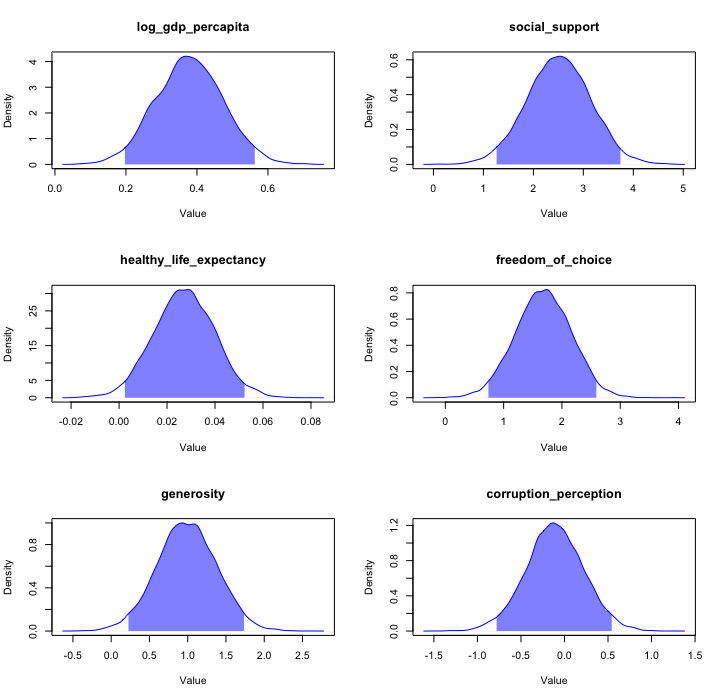
\includegraphics[scale=.7]{distributions.png}
\caption{\label{fig:dist-basic}Parameter distributions, classical regression}
\end{figure}

\begin{samepage}
\pagebreak
\subsection{Residual Plot}
\begin{figure}[h!]
\centering
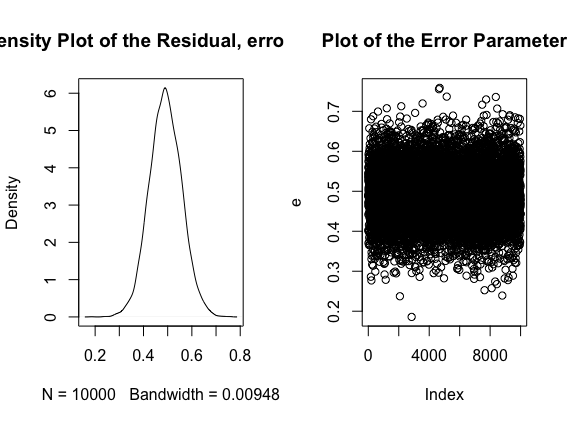
\includegraphics[scale=.6]{Rsidual.png}
\caption{\label{fig:pred} Prediction error}
\end{figure}
\end{samepage}

\begin{samepage}
\subsection{Cleaned Data for Longitudinal Model} \label{sec:apx_long_data}

\begin{table}[h!]
\centering
\caption{\label{tab:long_clean}10 happiest countries, data prepared for longitudinal analysis}
\begin{tabular} {l}
\hline
    \DTLloaddb{happy_data}{./data/happiest_clean.csv}
	\DTLdisplaydb{happy_data}
  \\ \hline
    $^1$ Measurement pulled-back from Switzerland 2009 survey results. \\
    $^2$ Measurement interpolated from Norway 2012, 2014 survey results. \\
    $^3$ Measurement interpolated from Switzerland 2012, 2014 survey results. \\
    $^4$ Measurement interpolated from Icleand 2013, 2015 survey results. \\ \hline
\end{tabular}
\end{table}
\end{samepage}

\end{document}